\section*{Results of the basic implementation of the
model}

2018/07/09 - SYNALP - Esteban MARQUER

\subsection{Paradigm}

The test is run on a minimal number of epoch (10), with a minimal model.

The training algorithm used is an example by example training.

\subsubsection{Model architecture}

The model is a line by line predictive model, composed of: - a character
embedding layer; - a pooling layer; - a linear layer; - an output layer.

The output of the model is a probability distribution over known
characters for every character of the predicted line.

\subsection{Results}

\subsubsection{GPU memory usage}

As expected from the model architecture, GPU memory usage is constant.

\begin{figure}[ht]
\centering
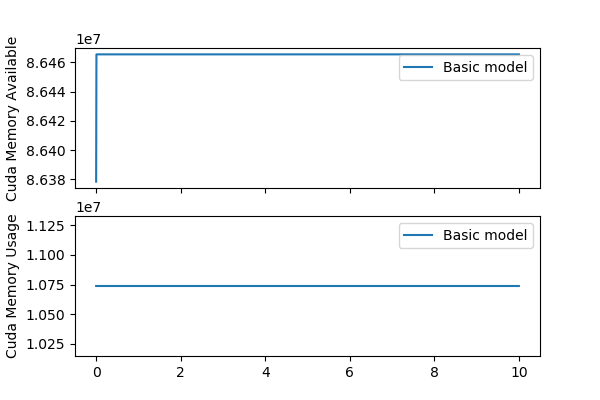
\includegraphics{parts/appendix/reports-papud/2018_07_09-Basic_implementation_results/memory.png}
\caption{memory usage}
\end{figure}

\subsubsection{Computation time}

\subsubsection{Loss and accuracy}

The loss used is cross-entropy loss, a character per character
negative-log-likelihood loss over the soft-maxed distribution.

Overall, the loss gives a score to the prediction of the model, by
comparing the target character and a distribution of probabilities for
each character. If the probability for the target character is high and
other character low, the model does a good prediction of the character,
and the score given is low. The closer the score is to 0, the better it
is. The scores of each characters is averaged, producing a global loss
over the line.

Accuracy is a percentage. The closer to 100 \% the better. As the loss
is bound by 0 and +Infinity, and the closer to 0 the better, a correct
transformation to accuracy could be: \lstinline!exp(-loss)! for an
accuracy between 0 and 1.

\begin{figure}[ht]
\centering
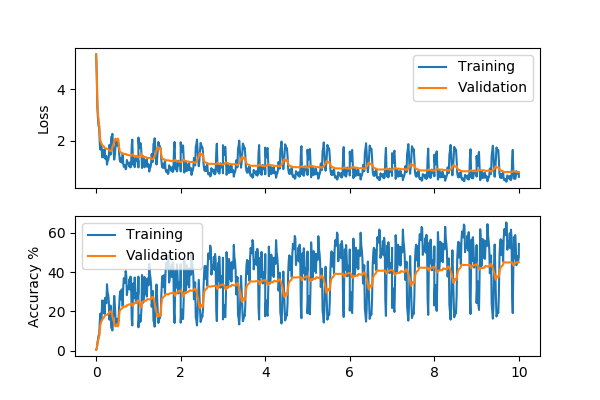
\includegraphics{parts/appendix/reports-papud/2018_07_09-Basic_implementation_results/loss.png}
\caption{loss}
\end{figure}

The small spike recurrently appearing in the loss and accuracy is most
likely due to a noisy part of the corpus (around the middle of the
corpus) causing the model to learn wrongly on those specific examples.

The best precision obtained at the end of 10 epochs is 50\%,
corresponding to a loss of about 0.7.

\subsection{Improvements and next
steps}

\subsubsection{Mini-batch}

Currently, the models learn one example at a time, meaning it computes
the result for a line of input, compares it to the target, and updates
weights. A common algorithm is the mini-batch algorithm, computing
simultaneously a set of examples, their loss compared to the target, and
updates the weights of the model all at once for the whole set of
examples.

This algorithm speeds-up training while making the most of the GPU.

\subsubsection{Dynamic corpus}

While with the current corpus there is no real problem in storing the
whole corpus in the memory, the future corpus will be over 400GB of
text. It is necessary to replace the current method by a dynamic loading
and transformation of the parts of the corpus currently used by the
model. An ideal solution would be to read the target data directly from
the archive containing the corpus.
